% Created 2021-12-03 Fri 11:17
% Intended LaTeX compiler: pdflatex
\documentclass[a4paper,openany]{tufte-book}
\usepackage[utf8]{inputenc}
\usepackage[T1]{fontenc}
\usepackage{graphicx}
\usepackage{longtable}
\usepackage{wrapfig}
\usepackage{rotating}
\usepackage[normalem]{ulem}
\usepackage{amsmath}
\usepackage{amssymb}
\usepackage{capt-of}
\usepackage{hyperref}
\usepackage{caption}
\usepackage[svgnames]{xcolor}
\usepackage{booktabs}
\usepackage{array}
\usepackage{tikz}
\usetikzlibrary{arrows,calc,decorations,shapes,shapes.arrows,shapes.misc,positioning,decorations.pathmorphing,patterns}
\usepackage{pgfplots}
\pgfplotsset{compat=1.16}
\usepackage{amsmath}
\usepackage{siunitx}
\usepackage{multirow}
\makeatletter
% Paragraph indentation and separation for normal text
\renewcommand{\@tufte@reset@par}{\setlength{\RaggedRightParindent}{0pt}  \setlength{\JustifyingParindent}{0pt}  \setlength{\parindent}{0pt} \setlength{\parskip}{\baselineskip}}
\@tufte@reset@par
% Paragraph indentation and separation for marginal text
\renewcommand{\@tufte@margin@par}{\setlength{\RaggedRightParindent}{0pt} \setlength{\JustifyingParindent}{0pt} \setlength{\parindent}{0pt} \setlength{\parskip}{\baselineskip}}
\makeatother
\author{Sappinandana Akamphon}
\date{\today}
\title{Mechanical Design}
\hypersetup{
 pdfauthor={Sappinandana Akamphon},
 pdftitle={Mechanical Design},
 pdfkeywords={},
 pdfsubject={},
 pdfcreator={Emacs 28.0.60 (Org mode 9.6)}, 
 pdflang={English}}
\usepackage{biblatex}
\addbibresource{/home/sup/ME310-2/me310-2.bib}
\begin{document}

\begin{titlepage}
  \newgeometry{top=1cm,left=1cm} %defines the geometry for the titlepage
  \pagecolor{Grey!50!Black}
  \includegraphics[scale=0.2]{pictures/logo-tu} \\
  \noindent
  \color{white}
  \makebox[0pt][l]{\rule{1.3\textwidth}{1pt}}
  \par
  \noindent
  \textbf{\textsf{Thammasat University}} \textcolor{yellow}{\textsf{Faculty of Engineering}}
  \vfill
  \hspace{1cm}
  \includegraphics[width=\textwidth]{pictures/gear-titlepage}
  \vfill
  \noindent
  \raggedleft{\Huge{ME 310: Mechanical Design}} \\
  \vspace{1cm}
  \raggedleft{\huge{Power Transmission}} \\
  \vspace{1cm}
  \noindent
  {\Large {Sappinandana Akamphon}}
\end{titlepage}

\restoregeometry
\nopagecolor

\frontmatter

\chapter{Preface}
\label{sec:org646a2a7}
This book is the second part of ME 310: Mechanical Design. In this book,
power transmission components are covered.

Sappinandana Akamphon

\tableofcontents

\listoffigures

\listoftables

\chapter{Revisions}
\label{sec:orgde501f4}
\subsubsection{September 2019}
\label{sec:orga3fa04b}

Start of Mechanical Design: Power Transmission

\subsubsection{January 2020}
\label{sec:org77d7a2d}

Began working on the chapters on shaft components, gears, brakes and clutches

\subsubsection{October 2021}
\label{sec:org68fdef9}

Completed chapters on gears, shafts,

\mainmatter

\chapter{Shaft and Shaft Components}
\label{sec:org631ce3d}

Most engineering systems are powered by rotational machinery such as internal combustion engines and electrical motors. It is, thus, extremely important that we understand and properly design power tranmission mechanism from the rotational machinery power source to intended components. Shafts remains one of the most prevalent methods of transmitting rotational power, and so it is our first chapter into the world of power transmission design.

By itself, shaft design is no more complex than other components under static or cyclic loadings already covered in the first book of this series. However, as shafts lie at the heart of most machine design applications, its final design will also depend on the design of other components that are to be mounted or connected to the shaft.

\section{Shaft Materials}
\label{sec:org9beaa8d}

There are two main concerns with designing a shaft: deflection and strength. Deflection is not affected by material strength. In fact, it depends only on the stiffness, represented by the Young's modulus. Since the Young's modulus is essentially the same for all steels, material choice matters little for deflection.

Strength, on the other hand, constitute a major concern for shaft design. Strength is necessary to resist loading stresses and fatigue stresses from the constant rotation. Many shafts are made from low carbon, cold-drawn or hot-rolled steel such as ANSI 1020-1050 steels. Significant strengthening from heat treatment or high alloy is often not neeeded. And fatigue failure is only reduced moderately by increase in strength, after a certain level notch sensitivity begins to counteract its benefit.

A good way to select a proper shaft material is to start with an inexpensive low or medium carbon steel for the first round of calculations. If strength considerations turn out to be the limiting factor over deflection, select a higher strength material and reduce the shaft size accordingly until deflection becomes an issue. The cost of the material and its manufacturing processes must be weighed against the need for smaller shaft diameter.

When additional strengthening is needed, typical alloy steels for heat treatment include ANSI 340-50, 3140-50, 4140, 4340, 5140, and 8650. Shafts don't usually need surface hardening unless there is significant risk of wear from journal bearing, in which case surface hardening include carburizing grades of ANSI 1020, 4320, 4820, and 8620. \autocite{shigley2011shigley}

\section{Shaft Layout}
\label{sec:org5a71f1c}

Generally a shaft is a cylinder with segments of varying cross sections
to accommodate components like gears, bearings, pulleys, etc. Shaft
shoulders are normally used to axially locate elements and to take any
axial thrust loads. illustrates the cross-section of a vertical
worm-gear speed reducer. In this figure, the shaft steps are used to
axially locate the two tapered bearings and the spur gear.

\begin{figure}[htbp]
\centering
\includegraphics[width=.9\linewidth]{pictures/Shafts/speed-reducer-layout.png}
\caption{A vertical worm-gear speed reducer. \emph{(Courtesy of the Cleveland Gear Company.)}}
\end{figure}

\section{Axial Layout of Components}
\label{sec:org79a60e6}

The axial positioning of components is often preset by the layout of the
housing and other meshing components. Generally it is advisable to
support any loading-carrying components between bearings. (TODO: NEED
FIGURE) However, pulleys and sprockets tend to be mounted outside of the
bearing pairs for ease of installation of the belt or chain. The length
of the shaft should be kept as short as possible to minimize deflection
and resultant load on the bearings.

In most cases, a shaft will only require two bearings, but in cases with
long shafts carrying multiple load-carrying components, it may be
necessary to use more than two bearings for additional support. In such
a case, particular care must be given to the alignment of the bearings.

\section{Supporting Axial Loads}
\label{sec:org5043fff}

There are use cases where axial loads in shaft may be significant, in
which case it is important to provide a means to transfer the axial
loads into the shaft. The shaft would then transfer the loads to a
bearing and to the ground. This is necessary for shafts mounted with
components that generate axial loads like bevel and helical gears, or
tapered roller bearings.

It is usually sufficient to have only one bearing carry the axial load.
This allows for greater tolerances on shaft length dimensions and
prevents binding from shaft thermal expansions, which is especially
significant in long shafts. TODO: figures showing shaft that carries
axial loads.

\section{Support for Torque Transmission}
\label{sec:org1d8d603}

Most shafts serve to transfer torque from an input (gear, pulley,
engine, motor, etc.) to an output gear or pulley. The shaft must be
sized to support torsional stress and its resultant angle of twist. It
is also important to provide a way to transmit the torque between the
gear (or pulley) and the shaft itself. Common torque transfer methods
are:

\begin{itemize}
\item Keys
\item Splines
\item Setscrews
\item Pins
\item Press or shrink fits
\item Tapered fits
\end{itemize}

There are also shafts that are designed to fail if excessive torque is
applied, to prevent failure of more expensive components. Details of the
components and their design process is covered in .

\section{Shaft Design for Stress}
\label{sec:orge0d8bcc}

It is not always necessary to evaluate stresses at every point; the same
goes for shafts as well. Only a few potentially critical locations
should be more than enough. Since the main types of load on shafts are
torsion and bending, it follows that most critical locations on the
shafts are on the outer surface--typically where the bending moment is
large, the torque is large, and where stress concentrations exist.

In order to determine the bending moments, torques, and shear forces on
a shaft, it is usually a good idea to draw shear and bending moment
diagrams. Since most shafts are loaded by gears and pulleys, introducing
forces in two planes, two diagrams are needed to determine the loads.
Resultant moments can be obtained simply by adding the moments as
vectors at points of interest. The normal stress due to bending will be
highest on the outer surfaces and will contribute to fatigue on a
rotating shaft.

Axial stresses on shafts from axial loads caused by helical gears or
tapered roller bearings are typically negiligible compared to the
bending stress. The axial stresses are also usually constant, meaning
that they rarely contribute significantly to fatigue. However, axial
stresses resulting from axial loads applied through other means should
be explicitly considered.

Let us now consider the shaft stresses, which are usually the
combination of normal stresses from bending and axial stresses, and
shear stress from torsion.

\begin{align}
  \label{eq: shaft normal and shear stresses}
  \begin{array}{ll}
    \sigma_a = K_f \dfrac{M_a y}{I} & \sigma_m = K_f \dfrac{M_m y}{I} \\[1em]
    \tau_a = K_{fs} \dfrac{T_a r}{J} & \tau_m = K_{fs} \dfrac{T_m r}{J}
  \end{array}
\end{align}

If we assume a solid shaft with circular cross section, we can further
simplify the expression to

\begin{align}
  \label{eq: shaft normal and shear stresses simplify}
  \begin{array}{ll}
    \sigma_a = K_f \dfrac{32M_a}{\pi d^3} & \sigma_m = K_f \dfrac{32M_m}{\pi d^3} \\[1em]
    \tau_a = K_{fs} \dfrac{16T_a}{\pi d^3} & \tau_m = K_{fs} \dfrac{16T_m }{\pi d^3}
  \end{array}
\end{align}

The stresses can be combined into stress amplitude and average stress
using maximum distortion energy theory (MDET or von Mises) as

\begin{align}
  \label{eq: von mises shaft stress}
  \sigma_{ae} &= \left( \sigma_a^2 + 3\tau_a^2 \right)^{1/2} = \left[ \left( \dfrac{32 K_fM_a}{\pi d^3} \right)^2 + 3\left( \dfrac{16 K_{fs} T_a}{\pi d^3} \right)^2 \right]^{1/2} \\
  \sigma_{me} &= \left( \sigma_m^2 + 3\tau_m^2 \right)^{1/2} = \left[ \left( \dfrac{32 K_fM_m}{\pi d^3} \right)^2 + 3\left( \dfrac{16 K_{fs} T_m}{\pi d^3} \right)^2 \right]^{1/2}
\end{align}

The stress concentration factors for the average stress component in
ductile materials can sometimes be ignored since the materilas can yield
locally at the discontinuity.

These equivalent stresses can be evaluated in design equations to
determine the safety factor \(N_s\) or the required diameter \(d\) using
the the modified Goodman diagram as

\begin{align}
  \frac{1}{N_s} = \frac{\sigma_{ae}}{S_e} + \frac{\sigma_{me}}{S_{ut}}
\end{align}

Substituting for \(\sigma_{ae}\) and \(\sigma_{me}\) results in

\begin{align}
  \frac{1}{N_s} = \frac{16}{\pi d^3} \left\{ \frac{1}{S_e} \left[ 4 \left( K_f M_a \right)^2 + 3 \left( K_{fs} T_a \right)^2 \right]^{1/2} + \frac{1}{S_{ut}} \left[ 4 \left( K_f M_m \right)^2 + 3 \left( K_{fs} T_m \right)^2 \right]^{1/2} \right\}
\end{align}

The required diameter \(d\) can be solved from the previous equation as

\begin{align}
  d = \left( \frac{16N_s}{\pi} \left\{ \frac{1}{S_e} \left[ 4 \left( K_f M_a \right)^2 + 3 \left( K_{fs} T_a \right)^2 \right]^{1/2} + \frac{1}{S_{ut}} \left[ 4 \left( K_f M_m \right)^2 + 3 \left( K_{fs} T_m \right)^2 \right]^{1/2} \right\} \right)^{1/3}
\end{align}

In many applications, rotating shafts will be under constant bending and
torsion, resulting in completely reverse bending stress (\(M_m = 0\))
and constant torsional shear stress (\(T_a = 0\)). This means the
required diameter becomes

\begin{align}
  d = \left( \frac{16N_s}{\pi} \left\{ \frac{2 K_f M_a}{S_e} + \frac{\sqrt{3} K_{fs} T_m}{S_{ut}} \right\} \right)^{1/3}\end{align}

\subsection{Example: Shaft sizing}
\label{sec:orgc5aa999}

\begin{center}
\includegraphics[width=.9\linewidth]{./pictures/Shafts/shaft-sizing.png}
\end{center}

Size the shaft (AISI 1040, \(S_{y}\) = 400 MPa, \(S_{ut}\) = 600 MPa)
using

\begin{enumerate}
\item MDET

\item Soderberg theory
\end{enumerate}

so that the safety factor \(N_{s}\) = 3.

\subsection{Solution}
\label{sec:org51c2c88}

\begin{enumerate}
\item MDET: The torque loaded on the pulley by the belt is

\begin{align*}
T &= (2020-20)(0.1) \\
&= 200.0\text{ N-m}
\end{align*}

There is also 2040 N of force pulling at the pulley due to the combined
belt tension. The torque generates shear stress throughout the shaft,
with the maximum value at the surface. The belt tension creates
bending stresses, whose maximum values are are the top and bottom of
the shaft at the middle. This means that the critical points on the
shaft (without considering stress concentration from the key/keyseat)
are at the top and bottom of the shaft at the middle. In this
problem, we will take the bottom of the shaft at the middle. The
stress concentration of the keyseat is taken to be \(K_{f}\) = 2.14
in bending and \(K_{fs}\) = 3.0 in torsion.

\begin{align*}
\sigma &= K_{f}\frac{My}{I} = 2.14\frac{ 2040(0.6)(r)}{4 \pi r^{4}/4} \\
&= \frac{834}{r^{3}} \text{ Pa} \\
\tau &= K_{fs}\frac{Tr}{J} = 3\frac{(200.0)(r)}{\pi r^{4}/2} \\
&= \frac{382}{r^{3}} \text{ Pa}
\end{align*}

\item Soderberg: using the criteria, we must calculate the minimum and maximum bending moments and torques, which will then be used to determine the stress amplitudes and average stresses. We already determine the maximum bending moment and torque, which we used to determine the corresponding stresses for MDET. We now only need to find out the minimum bending moment and torque. The minimum bending moment occurs when the shaft rotates by half a revolution, for which the beam willbe under a compressive stress of the same magnitude.

\begin{align*}
\sigma_{\min} &= -\frac{834}{r^{3}} \\
\sigma_{a} &= \frac{\sigma_{\max} - \sigma_{\min}}{2} \\
&= \frac{834}{r^{3}}
\end{align*}

If the shaft is under continuous operation, the applied torque is constant, which means that the torque amplitude \(T_{a}\) = 0 and the average torque \(T_{m} = T\). We can plug this into the sequation to determine equivalent amplitude and average stresses.

\begin{align*}
\sigma_{ae} &= \sqrt{ \sigma_{a}^{2} + 3 \tau_{a}^{2} } = \frac{834}{r^{3}} \\
\sigma_{me} &= \sqrt{ \sigma_{m}^{2} + 3 \tau_{m}^{2}} = \frac{662}{r^{3}} \\
\frac{1}{3} &= \frac{834}{0.5(\num{6.00e+08})r^{3}} + \frac{662}{\num{4.00e+08}(r^{3})} \\
r &=0.0237\text{ m}
\end{align*}

Using the settings from the previous example, redetermine the shaft size if the maximum operating speed is 10000 rpm.
\end{enumerate}


For a simply supported shaft, the first natural frequency that can cause shaft whirling is

\begin{align}
  \omega_{1} = \left( \frac{\pi}{l} \right)^{2} \sqrt{ \frac{EI}{A \rho} }
\end{align}

We must first convert the angular velocity into rad/s: 10000 rpm = 10000(2\(\pi\)/60) = rad/s. To achieve the safety factor of 3, the first natural frequency of the shaft must be

\begin{align*}
\omega_{1} &=3(1047) = \left( \frac{\pi}{0.6} \right)^{2} \sqrt{ \frac{\num{2.10e+11} \pi r^{4}/4 }{\pi r^{2} \rho}} \\
r &=0.044\text{ m}
\end{align*}

The designed shaft has to follow the largest shaft that satisfy each of the condition, therefore the required radius is 4.4 cm.

\section{Torque Trasmission Components}
\label{sec:orgb36f3a5}

For a designed shaft to properly transfer torque to its intended target, not only must the shaft be able to with stand the stresses resulting from the torque, but it must also be assembled with torque transmission components that are capable of transferring such torque. Some of the mechanisms currently in use can be categorized into:

\begin{enumerate}
\item Mechanical drive assembly
\item Interference fit assembly
\item Welded assembly
\end{enumerate}

\subsection{Mechanical Drive Assembly}
\label{sec:orgb300850}

Mechanical drive assembly typically requires adjustments to the shaft and/or hub of the component to be assembled. The most common mechanical-drive assembly is the conventional key and keyway. Other assemblies are set screws, pins, and spline shafts.

\subsubsection{Keys and Pins}
\label{sec:org5b9928e}

Keys are axially inserted metal that provides interference between the shaft and hub, allowing torque trasmission between the two. Aligning keyways need to be cut into both the shaft and the hub.

Pins, on the other hand, are transversely inserted perpendicular to the axis of the shaft. Both the shaft and hub still needs to be drilled.

\begin{center}
\includegraphics[width=.9\linewidth]{./pictures/Shafts/keys-pins.png}
\end{center}

While pins allow for torque transmission and axial positioning, keys only allow torque transmission. However, because of the typical long length of keys inserted axially which provides larger cross-sectional area, they typically allow larger torque trasmission than pins of the same size.

Torque capacity of keys and pins can be calculated by

\begin{align*}
  P_{\max} &= \frac{S_{y}}{\sqrt{3}}A = 0.577 S_{y}A \\
  T_{\max} &= P_{\max}r_{\text{shaft}}
\end{align*}

\section{Limitation of Mechanical Drive Assembly}
\label{sec:org55da26c}

Mechanical drive assembly can provide relatively high torque transmission with relatively easy assembly. However, they have a few shortcomings to consider.

\begin{enumerate}
\item Stress concentration: shafts and hubs need to be machined to provide holes/keyways/splines, which will obviously introduce increased stress concentration and thus reduced shaft/hub strength.

\item Backlash: even with very strict tolerances, pins and keys that do not perfectly fit in the holes or keyways will allow relative motion between the shaft and the hub, leading to backlashes. However, this can be eliminated or mitigated with the use of tapered keys or pins.

Tapered keys or pins have a slowly increasing cross section from one end to the other, therefore allowing a snug fit.

\item Machining costs: as keyways/splines/holes require precise machining, this will incur additional costs on the shaft assembly.

\item Uneven distribution of mass: uniform distribution of mass about the shaft is extremely important for shaft stability especially in high speed application. Usually components such as gears, pulleys, sprockets, etc. are designed to be axisymmetric for this reason. However, the required machining and insertion of keys or pins will introduce asymmetry to the shaft assembly.
\end{enumerate}

\subsection{Example: Key Sizing}
\label{sec:org8c7cf6f}

A steel shaft whose \(S_y\) = 450 MPa has a diameter of 5 cm. The shaft rotates at 600 rpm and transmits 40 hp through a gear. Select an appropriate key for the gear. Use safety factor = 3.

\begin{figure}[htbp]
  \centering
  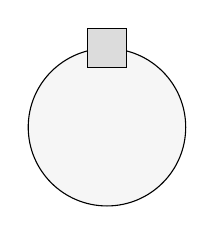
\begin{tikzpicture}
    \node[circle, draw, fill=LightGrey!20, minimum height=2cm](shaft){};
    \node at (shaft.north) [draw, fill=LightGrey!80, minimum height=5mm, minimum width=5mm](key){};
  \end{tikzpicture}
\caption{Key and shaft cross section for example \ldots{}}
\end{figure}

\subsection{Solution: Key Sizing}
\label{sec:org7ea0a16}

To keep things simple, pick a square key and pick key length = 2 cm.

\begin{align*}
  T &= \frac{H}{\omega} = \frac{40(746)}{600(2\pi/60)} \\
    &= 475 \text{ N-m}
\end{align*}

For the width (and height) of the key section,

\begin{align*}
  N_{s} T_{\max} &= 0.577S_{y}blr_{\text{shaft}} \\
  b &= \frac{3(475)}{0.577(450 \times 10^{6})(0.02)(0.05)} \\
  b &= 0.00549 \text{ m}
\end{align*}

\section{Interference Fit Assemblies}
\label{sec:org213f72f}

Interference fit refers to a type of joint that relies on friction between the hub and shaft to transfer torque. The friction results from the compression of the hub on the shaft, which means the diameter of the hole on the hub must be slightly smaller than that of the shaft. These type of assemblies are divided into 3 categories based on method of assembly.

\begin{enumerate}
\item Press fit:

The word 'press' here refers to the assembly method of pressing the shaft into a hole that is slightly smaller. This process relies on the elasticity of both materials to allow the shaft to slide in without any permanent deformation. This requires extremely strict tolerances on both the shaft and the hub.

\item Tapered fit:

In case of tapered fits, an additional collet, which is a collar that is tapered on the outside along the length, and has a constant cross section on the inside. The collet essentially acts like a wedge between the shaft and hub, allowing the assembler to control the magnitude of compressive (and resulting friction) force on the shaft by the axial load exerted on the collet.

\item Shrink fit:

Similar to press fit in that there is no additional 'collet', but instead of 'pressing' the shaft onto the hub, either the shaft is cooled or the hub is heated (or both) before assembly. This eliminates the difficulty of assembly and allows for greater difference in the diameters of the shaft and hub.
\end{enumerate}

These interference fits do not require any machining on the shaft or hub, thus do not increase the stress concentration nor incur additional machine costs. However, they do have the following limitations to take into consideration.

\begin{enumerate}
\item Materials, surface, and design restrictions: interference fits rely on friction, so the material, surface finishing, and shaft dimensions (diameter mostly) affect the magnitude of friction that can be generated. This limits your available choices.

\item Close tolerance: interference fits require that the hubs and shafts have extremely close and accurate tolerances, requiring precise machining. This leads to high machining costs.

\item Fretting: high stress on surfaces that undergo repeated motions are prone to fretting corrosion.

\item Surface galling: high compressive load on mating surfaces can cause them bind. This complicates dissasembly, which usually results in surface failure.

\item High stress in components: interference fit requires high compressive force from the hub on the shaft to generate friction. This leads to circumferential stresses on the hub and the shaft as well.
\end{enumerate}

\section{Stresses in Interference Fits}
\label{sec:org36e6be2}

Assumed uniform pressure on shaft (i) and hub (o)

\begin{align*}
  p &= \frac{d_{\text{shaft}} - d_{\text{hub}}}{\dfrac{d}{E_{o}} \left( \dfrac{d_{o}^{2} + d^{2}}{d_{o}^{2} - d^{2}} + \nu_{o} \right) + \dfrac{d}{E_{i}}\left( \dfrac{d^{2} + d_{i}^{2}}{d^{2} - d_{i}^{2}} - \nu_{i} \right)}
\end{align*}

When both are of the same material

\begin{align*}
  p &= \frac{E(d_{\text{shaft}} - d_{\text{hub}})}{2d^{3}} \left[ \frac{(d_{o}^{2} - d^{2})(d^{2} - d_{i}^{2})}{d_{o}^{2} - d_{i}^{2}} \right]
\end{align*}

Tangential and radial stresses in shaft and hub are

\begin{align}
  \sigma_{t,\text{shaft}} &= -p \frac{d^{2} + d_{i}^{2}}{d^{2} - d_{i}^{2}} \\
  \sigma_{t,\text{hub}} &= p \frac{d_{o}^{2} + d^{2}}{d_{o}^{2} - d^{2}} \\
  \sigma_{r,\text{shaft}} &= -p \\
  \sigma_{r,\text{hub}} &= -p
\end{align}

Combine \(\sigma_{t}\) and \(\sigma_{r}\) using MDET to determine failure

\section{Torque Capacity of Interference Fits}
\label{sec:org2f350b8}

Depends on friction generated between shaft and hub \(\rightarrow\) pressure from interference fits

\begin{align}
  f &= \mu N = \mu (pA) \nonumber \\
    &= \pi \mu pld \\
  T &= fd/2 = \pi \mu pld(d/2) \nonumber \\
    &= \frac{\pi}{2}\mu pld^{2}
\end{align}

\subsection{Example: Torque Capacity of an Interference Fit}
\label{sec:org04535a7}

A solid shaft whose diameter is 5 cm is pressed onto a gear whose hub inner diameter is 4.99 cm and outer diameter is 6 cm. If both are made of the same steel whose \(E\) = 210 GPa and \(\nu\) = 0.3, determine the radial and tangential stresses, along with the torque capacity of the fit. Assume steel-on-steel \(\mu\) = 0.3, and the hub is 7 cm long.

\subsection{Solution: Torque Capacity of an Interference Fit}
\label{sec:orgba8b0c8}

\begin{align*}
  p &= \frac{E(d_{\text{shaft}} - d_{\text{hub}})}{2d^{3}} \left[ \frac{(d_{o}^{2} - d^{2})(d^{2} - d_{i}^{2})}{d_{o}^{2} - d_{i}^{2}} \right] \\
    &= \frac{210 \times 10^{9} (0.05 - 0.0499)}{2(0.05)^{3}} \left[ \frac{(0.06^{2} - 0.05^{2})(0.05^{2} - 0)}{0.06^{2} - 0} \right] \\
    &= 64.2 \text{ MPa} \\
  \sigma_{r,\text{shaft}} &= \sigma_{r,\text{hub}} = -64.2 \text{ MPa} \\
  \sigma_{t,\text{shaft}} &= -64.2 \frac{0.05^{2}}{0.05^{2}} = -64.2 \text{ MPa} \\
  \sigma_{t,\text{hub}} &= 64.2 \frac{0.06^{2} + 0.05^{2}}{0.06^{2} - 0.05^{2}} = 356 \text{ MPa} \\
  T &= \frac{\pi}{2}\mu pld^{2} = \frac{\pi}{2}(0.3) 64.2 \times 10^{6} (0.07)(0.05^{2}) = 5294 \text{ N-m}
\end{align*}


\section{Weld Assembly}
\label{sec:orgf37ecd1}

In weld assemby, the shaft and hub of intended components are welded together. This provides a relatively quick and permanent connection between the components. However, weld assemblies also inherit the same disadvantages from welded joints as mentioned in chapter \ldots{}.

\begin{enumerate}
\item Welding only works on compatible materials. Plastics on metals is a no-no. Woods cannot be welded. Ceramics cannot be welded. You get the idea.

\item Heating can cause warpage. Welding introduces uneven heating of the workpiece, which can result in warpage especially in parts with complex geometries.

\item Disassembly. Welding is permanent\ldots{} mostly. Welding can be undone, although the process is not straightforward and can cause permanent surface damages.

\item Skilled personnel. Welding requires skilled craftmanship, which means it is usually expensive and its quality is hard to control.

\item Cleaning and machining. Welding typically needs cleaning and machining afterwards to obtain desirable surface finish.
\end{enumerate}

\section{Torque Capacity in Weld Assembly}
\label{sec:org5b03c64}

The strength of weld can be applied to determine the torque capacity of shafts and their components in weld assembly. In most cases, weld joints in weld assembly are fillet welds and the corresponding equations apply.

\chapter{Journal Bearings and Lubrication}
\label{sec:org3167d49}

\section{Overview of Bearings}
\label{sec:org486d33b}

\section{What are bearings?}
\label{sec:org42e6a4b}

\begin{itemize}
\item A feature that allows relative motions between components

\begin{itemize}
\item Linear motions

\item Rotary motions
\end{itemize}
\end{itemize}

\section{Two types of bearings}
\label{sec:org714bc6b}

\begin{itemize}
\item Contact: sliding or rolling

\item Non-contact: fluid film or magnetic
\end{itemize}

\chapter{Contact Bearings}
\label{sec:org1797ea2}

Contact bearings are features that allow relative movements between two surfaces wherein the surfaces remain in contact with each other either directly or indirectly through some solid common medium.


\section{Sliding Contact Bearings}
\label{sec:org41c7d89}

\begin{figure}[htbp]
\centering
\includegraphics[width=.9\linewidth]{./pictures/Bearings/sliding-contact-bearing.jpg}
\caption{Brass sliding contact bearing}
\end{figure}

\begin{itemize}
\item Commonly used in low- to medium-speed applications
\end{itemize}


\begin{itemize}
\item Lubrication is used to reduce wear and friction
\end{itemize}

\section{Materials for Sliding Contact Bearing}
\label{sec:org3e6ef6a}

\begin{itemize}
\item Typically hard materials (shaft) on soft (bearing)

\item Materials:

\begin{itemize}
\item Polymers: nylon is king!

\item Brass

\item Ceramics
\end{itemize}

\item Check on bearing stress

\item Aluminum-on-aluminum is a no-no
\end{itemize}

\section{Bearing Contact Pressure}
\label{sec:orgea61431}

\begin{align}
  P &= \frac{F}{DL} \\
  P_{\max} &= \frac{4}{\pi} \frac{F}{DL}
\end{align}

\section{PV Factor}
\label{sec:org8f7b616}

In selecting materials for sliding-contact bearings.

\begin{itemize}
\item pressure \(\times\) velocity

\item tradeoff in choosing bearing materials

\item higher pressure \(\rightarrow\) low speed, and vice versa
\end{itemize}

\begin{figure}[htbp]
\centering
\includegraphics[width=.9\linewidth]{./pictures/Bearings/pv-metal.png}
\caption{PV Table for Metals}
\end{figure}


\begin{figure}[htbp]
\centering
\includegraphics[width=.9\linewidth]{./pictures/Bearings/pv-nonmetal.png}
\caption{PV Table for Nonmetals}
\end{figure}


\section{Example: Sleeve Bearing for a Low-speed Shaft}
\label{sec:org31fe17b}

A 30-cm long shaft whose diameter \(D\) is 3 cm is operated at 1000 rpm.
The shaft has a spur gear whose \(R_{\text{pitch}}\) = 10 cm mounted in
the middle with a bearing at each end. The gear is transferring the
power of 1.5 kW. The gear has pressure vessel \(\theta\) =
20\(^{\circ}\). Determine the minimum bearing length \(L\) using nylon.

\section{Solution}
\label{sec:orgf299c6a}

First, let us determine the force on the bearing. Since spur gears don't
generate any axial load, the forces will simply be the radial +
tangential load, perpendicular to the shaft.

\begin{align}
    T &= \frac{P}{\omega} \\
      &= \frac{1500}{1000(2\pi / 60)} = 14.3 \text{ N-m} \\
    F &= \frac{T}{R_{\text{pitch}} \cos \theta} \\
      &= \frac{14.3}{0.1 \cos 20^{\circ}} = 152 \text{ N}
\end{align}

Since the gear is mounted in the middle, the force on each bearing is
half of the force.

\begin{align}
    F_{bearing} = \frac{152}{2} = 76 \text{ N}
\end{align}

We can't determine the bearing pressure yet since we don't know the
bearing length. We can determine the surface velocity, however.

\begin{align}
    v = \omega (D/2) = 1000 (2\pi / 60) (0.03/2) = 1.57 \text{ m/s}
\end{align}

We double-check that \(v < V_{nylon} (1.57 < 3.0)\) so nylon is an
acceptable choice. The length of bearing, then should be

\begin{align}
  P_{bearing}v &< (PV)_{nylon} \\
  \frac{F_{bearing}}{DL}v &< 0.11 \times 10^6 \\
  \frac{76}{0.03L} 1.57 &< 1.1 \times 10^5 \\
  L &> 0.036 = 3.6 \text{ cm}
\end{align}

\chapter{Rolling Contact Bearings}
\label{sec:orgc476af0}
\section{Rolling Elements}
\label{sec:orgd10ed09}

\begin{itemize}
\item suitable for medium- to high-speed applications

\item use balls or rollers to avoid friction
\end{itemize}

\section{Rolling Element Types}
\label{sec:org1235670}

\begin{figure}[htbp]
\centering
\includegraphics[width=.9\linewidth]{./pictures/Bearings/bearing-series.png}
\caption{Bearing Series}
\end{figure}

\begin{figure}[htbp]
\centering
\includegraphics[width=.9\linewidth]{./pictures/Bearings/bearing-table.png}
\caption{Bearing table}
\end{figure}

\section{Bearing Life Requirement}
\label{sec:orge7be770}

\begin{align}
    L &= L_R K_r \left( \frac{C}{F_e} \right)^{10/3} \\
    C &= F_e \left( \frac{L}{K_r L_R} \right)^{0.3}
\end{align}

\begin{center}
\begin{tabular}{ll}
\(L\) & life corresponding to equivalent load \(F_e\)\\
\(L_R\) & life corresponding to rated capacity = 9 \(\times\) 10\(^7\) rev\\
\(K_r\) & reliability factor\\
\(C\) & rated capacity\\
\(F_e\) & equivalent load\\
\end{tabular}
\end{center}


\begin{figure}[htbp]
\centering
\includegraphics[width=.9\linewidth]{./pictures/Bearings/bearing-rated-capacity.png}
\caption{Bearing rated capacity \(C\)}
\end{figure}

\begin{figure}[htbp]
\centering
\includegraphics[width=.9\linewidth]{./pictures/Bearings/reliability-factor.png}
\caption{Bearing reliability factor \(K_r\)}
\end{figure}


\section{Equivalent Load}
\label{sec:orgf268461}
Let \(e = F_a / F_r\)

for radial ball bearings

\begin{align}
    F_e = \left\{
    \begin{array}{ll}
        F_r & e < 0.35 \\
        F_r \left[ 1 + 1.115(e - 0.35) \right] & 0.35 < e < 10 \\
        1.176 F_a & e > 10
    \end{array}
    \right.
\end{align}

for angular ball bearings

\begin{align}
    F_e = \left\{
    \begin{array}{ll}
        F_r & e < 0.68 \\
        F_r \left[ 1 + 0.87(e - 0.68) \right] & 0.68 < e < 10 \\
        0.911 F_a & e > 10
    \end{array}
    \right.
\end{align}

\section{Typical Bearing Design Life}
\label{sec:org3bab568}


\subsection{Radial Ball Bearing Selection}
\label{sec:org702fa13}

Select a radial ball bearing for a shaft intended for a continuous
8-hr-a-day operation at 1800 rpm with 95\% reliability. Axial and radial
loads are 1.2 kN and 1.5 kN, respectively.

\subsection{Solution}
\label{sec:orgc2e6efa}

First, we need to calculated \(F_e\).

\[e = \frac{F_a}{F_r} = \frac{1.2}{1.5} = 0.8\]

For radial ball bearing,

\begin{align}
  F_{e} &= F_r \left[ 1 + 0.87(e - 0.68) \right] \\
        &= 1500 \left[ 1 + 1.115(0.8 - 0.35) \right] \\
        &= 2276 \text{ N}
\end{align}

Required life for 8-hr-a-day service (assumed every day) = 30000 hrs

Life in revolutions

\[L = 1800(30000)(60) = 3.24 \times 10^9 \text{ revolutions}\]

For 95\% reliability \(K_r\) = 0.63

\begin{align}
    C = 2276 \left( \frac{3.24 \times 10^9}{0.63 (9 \times 10^7)} \right)^{0.3} = 7661 \text{ N} = 7.66 \text{ kN}
\end{align}

For extra-light, light, and medium series, the required bore are 55, 35,
and 30 mm, respectively

The models corresponding to the bore are L11, 207, and 306,
respectively.

\chapter{Gears}
\label{sec:org8e87974}
\section{Gear Overview}
\label{sec:org925ce4c}

Why Gears?

\begin{itemize}
\item Convert high speed and low torque to that requires low speed and high
torque

\item Speed: easy to get because voltage is easy

\item Torque: hard to get because it requires large current
\end{itemize}

Principles of Gears

\begin{itemize}
\item Allow positive engagement between teeth

\item High forces can be transmitted while in rolling contact

\item Do not need friction to operate
\end{itemize}

Basic Law of Gearing

\begin{itemize}
\item Point of contact between two mating gears is always the same relative
distances from the two centers.

\item Any gear tooth profiles that follow the law of gearing will result in
constant relative speed of rotation
\end{itemize}

Gear Geometry

Module of a Gear, \(m\)

\begin{itemize}
\item Term used to define gear tooth size

\item Defined as ratio of pitch diameter to number of teeth
\begin{align}
            m = \frac{D_{\text{pitch}}}{z}
          \end{align}

\item A pair of meshing gears must have the same modules!
\end{itemize}

Gear Types

Gear Terminology

\begin{description}
\item[{Pinion}] smaller of two gears, usually driving

\item[{Gear}] Larger of the two. Also called \emph{wheel}. Usually driven.
\end{description}

Gear Materials

\begin{itemize}
\item Steel: medium-carbon steel + heat treatment + grinding

\item Cast iron: surface fatigue > bending fatigue

\item Nonferrous: bronzes \(\rightarrow\) corrosion + wear resistant, low
friction

\item Nonmetallic: Nylon \(\rightarrow\) low friction and weight + corrosion
resistant, but low thermal conductivity
\end{itemize}

Gear Efficiency

\begin{itemize}
\item With friction, gears are 90 - 95\% efficient because of mostly rolling
contact

\begin{align}
  T_{\text{out}} &= \frac{\eta T_{\text{in}} d_{\text{out}}}{d_{\text{in}}} \\
  \omega_{\text{out}} &= \frac{\omega_{\text{in}} d_{\text{in}}}{d_{\text{out}}} \\
  P_{\text{out}} &= T_{\text{out}} \omega_{\text{out}}
\end{align}
\end{itemize}

\section{Gear Trains}
\label{sec:org979ffce}

Gear Trains When large reduction is required

\begin{itemize}
\item Large gear + small pinion: simple, but large stress and interference

\item Multiple pairs of gears and pinions: less simple, low stress, large
space

\item Planetary gears: complex, low stress, small space
\end{itemize}

Normal Gear Trains

\begin{align}
    e_{total} &= e_{1}e_{2}\cdots \\
  \end{align}

Planetary/Epicyclic Gear Train

\begin{itemize}
\item Planetary or epicyclic gears enable a high reduction ratio in small
spaces
\end{itemize}

Planetary Gear Components

Planetary Gears: Torque, Forces, and Reduction Ratios

\begin{itemize}
\item Symmetry \(\rightarrow\) no net force on shaft

\item Multiple planet gears reduce individual torque/force

\item Any combination of fixed, input, output gears

\item 1 gear box -> multiple gear reduction ratios
\end{itemize}

Fixed ring:\\

\begin{align}
  \omega_{\text{carrier}} &= 9 \\
  \omega_{\text{planet}} &= (9) \frac{60/2 + 20/2}{20/2} = 36 \\
  \omega_{\text{sun}} &= (36) \frac{20}{30} = 24 \\
  e &= 9/24 = 0.375
\end{align}

\begin{center}
\begin{tabular}{llrlr}
Fixed & Input & Planet & Output & RR\\
\hline
Ring & Carrier 9 & 36 & Sun 24 & 0.375\\
Sun & Carrier 9 & 36 & Ring 14.4 & 0.625\\
Carrier & Sun 9 & 27 & Ring 5.4 & 1.667\\
\end{tabular}
\end{center}

\chapter{Spur Gears}
\label{sec:org4702062}

Spur gears have straight involute teeth. They transfer torque by applying forces perpendicular to their involute face. And because their teeth are perpendicular to their axis, spur gears do not generate axial loads--they generate only tangential and radial forces.

\begin{align}
\label{eq: spur gear forces}
  F_{t} &= \frac{T}{R_{\text{pitch}}} \\
  F_{r} &= F_{t} \tan \phi \\
  F_{a} &= 0
\end{align}

The tangential force is perpendicular to gear teeth, leading to tooth bending

\section{Spur Gear Stress}
\label{sec:org6efb97d}

The equation for bending stress in spur gears is a modified lewis equation that takes into account the shapes, stress concentrations, and operating conditions of the gear.

\begin{itemize}
\item Bending Stress \(\rightarrow\) AGMA stress equation

\item Consider tooth as a cantilever beam
\end{itemize}

\begin{align}
  \sigma = \frac{F_{t}}{bY_{J}m} K_{O} K_{m} K_{v}
\end{align}

\begin{description}
\item[{\(F_{t}\)}] tangential force

\item[{\(b\)}] face width

\item[{\(Y_{J}\)}] geometry factor

\item[{\(m\)}] module
\end{description}

The geometry factor \(Y_J\) takes into account the involute shape and stress concentration factor of the tooth.

\begin{figure}[htbp]
\centering
\includegraphics[width=\textwidth]{./pictures/Gears/geometry-factor.png}
\caption{\label{fig: spur geometry factor}Geometry factor \(Y_J\) for spur gear design}
\end{figure}

From Figure \ref{fig: spur geometry factor}, gears with large number of teeth or that are mating with gears with large number of teeth have higher geometry factors, leading to lower bending stresses. This is because large number of teeth means the teeth are shorter, hence the lower stresses.

Overload Factor: \(K_{O}\)

This factor takes into account the shock and impact loading during operation, which can cause a sharp increase in the stress. We consider the source of shock and impact loading from both the power source (input) and the driven machine (output).

\begin{table}[htbp]
\caption{Overload factor \(K_O\) for spur gear design}
\centering
\begin{tabular}{lp{1.5cm}p{1.5cm}p{1.5cm}p{1.5cm}}
\toprule
\multirow{2}{*}{Power source} & \multicolumn{4}{c}{Driven Machine} &  &  & \\
 & Uniform & Light shock & Moderate shock & Heavy shock\\
\midrule
Uniform & 1.00 & 1.25 & 1.50 & 1.75\\
Light shock & 1.20 & 1.40 & 1.75 & 2.25\\
Moderate shock & 1.30 & 1.70 & 2.00 & 2.75\\
\bottomrule
\end{tabular}
\end{table}


Power sources can be categorized based on their shock/impact loading generated, along with some examples, as follows.

\begin{description}
\item[{Uniform}] Electric motor, constant-speed turbine

\item[{Light}] Water turbine, variable-speed drive

\item[{Moderate}] Multicylinder engine
\end{description}

Driven machines are categorized based on operating conditions, which depends mostly on the resisting load on the system.

\begin{description}
\item[{Uniform}] Continuous generator

\item[{Light}] Fans, low-speed pumps, conveyors

\item[{Moderate}] high-speed pumps, compressors, heavy conveyers

\item[{Heavy}] rock crushers, punch press drivers
\end{description}

Mounting Factor: \(K_{m}\)

The factor accounts for the increase in stress when tooth faces do not align perfectly. This can happen due to inaccurate mountings, the use of normal (rather than precision) gears, or off-center mountings.

\begin{center}
\begin{tabular}{p{6cm}cccc}
\toprule
\multirow{2}{6cm}{Characteristics of Support} & \multicolumn{4}{c}{Face Width (cm)} &  &  & \\
 & 0 to 5 cm & 15 & 22.5 & 40\\
\midrule
Accurate mountings, small bearing clearances, precision gears & 1.3 & 1.4 & 1.5 & 1.8\\
Less rigid moutings, standard gears, full face contact & 1.6 & 1.7 & 1.8 & 2.2\\
Less than full face contact & \multicolumn{4}{c}{Over 2.2} &  &  & \\
\bottomrule
\end{tabular}
\end{center}

Velocity Factor: \(K_{v}\)

This factor accounts for the increase in stress from increased pitch line velocity of the gears. This combines with the overloading factor \(K_O\) to describe the effect of shock and impact loading on stress.

\begin{align}
  K_{v} &= \left( \frac{A + \sqrt{200 v_{t}}}{A} \right)^{B} \\
  A &= 50 + 56(1 - B) \\
  B &= 0.25(12 - Q)^{2/3}
\end{align}

\begin{description}
\item[{\(v_{t}\)}] pitch line velocity [m/s]

\item[{\(Q\)}] AGMA Quality Number
\end{description}

\begin{marginfigure}
  \centering
  \begin{tikzpicture}
    \begin{axis} [
      width=\textwidth,
      height=0.75\textwidth,
      legend style={at={(0.75,0.25)},
        anchor=south east,legend columns=-1,
        fill=none},
      xlabel={$v_t$ [m/s]},
      xmin=0,xmax=30,
      ymin=1,ymax=2,
      ylabel={$K_v$},
      ]
      \addplot[domain=0:30]{(1 + sqrt(200*x)/(50 + 56*(1 - 0.25*(12 - 6)^(2/3))))^(0.25*(12-6)^(2/3))} node[midway, above left]{6};
      \addplot[domain=0:30]{(1 + sqrt(200*x)/(50 + 56*(1 - 0.25*(12 - 8)^(2/3))))^(0.25*(12-8)^(2/3))} node[midway, above left]{8};
      \addplot[domain=0:30]{(1 + sqrt(200*x)/(50 + 56*(1 - 0.25*(12 - 10)^(2/3))))^(0.25*(12-10)^(2/3))} node[midway, above left]{10};;
      \addplot[domain=0:30]{(1 + sqrt(200*x)/(50 + 56*(1 - 0.25*(12 - 12)^(2/3))))^(0.25*(12-12)^(2/3))} node[midway, above left]{12};;
    \end{axis}
  \end{tikzpicture}
\caption{Velocity factor \(K_v\) as a function of pitch line velocity \(v_t\) for various gear quality number \(Q\)}
\end{marginfigure}

AGMA recommends designers choose gears based on the level of precision they require from the deisgned mechanisms. Some of the guidlines are listed in Table \ref{tab: AGMA recommended quality}

\begin{table}[htbp]
\caption{\label{tab: AGMA recommended quality}AGMA recommended quality number for various applications}
\centering
\begin{tabular}{llp{5cm}}
\toprule
\(v_{t}\) [m/s] & \(Q\) & Applications\\
\midrule
0 - 4 & 6 - 8 & Paper box making machine, cement, mill drives\\
4 - 10 & 8 - 10 & Washing machine, printing press, computing mechanism\\
10 - 20 & 10 - 12 & Automotive transmission, Antenna drive, propulsion drive\\
\(\geqslant\) 20 & 12 - 14 & Gyroscope\\
\bottomrule
\end{tabular}
\end{table}

\subsection{Gear Material Strength \(S_e^{\prime}\)}
\label{sec:orgc35bfd4}

Because they are used exclusively in rotational machinery, gears are constantly under repeated loadings. Thus, their main mode of failure is fatigue. Hence, whenever we consider the strength of gear material for design, endurance limits should be the first factor on our list.
\begin{align}
  S_{e}^{\prime} = S_{e}C_{L}C_{G}C_{S}k_{r}k_{t}k_{ms}
\end{align}
where

\begin{description}
\item[{\(S_{e}\)}] endurance limit

\item[{\(C_{L}\)}] load factor (= 1 for bending)

\item[{\(C_{G}\)}] gradient surface = 1

\item[{\(C_{S}\)}] surface factor (= 0.75 for machined surface)

\item[{\(k_{r}\)}] reliability factor

\item[{\(k_{t}\)}] temperature factor

\item[{\(k_{ms}\)}] median-stress factor (1 for two-way bending (followers), 1.4 for one-way bending (input or output))
\end{description}

Now let us consider each of endurance limit modifier in more details.

Reliability Factor: \(k_{r}\)

Since most material properties--endurance limits included--are reported by their average values, obviously there will be a gear whose actual endurance limit is lower than the reported value. This reliability factor represents this probability so that a given design based on the reduced endurance limit will have a higher probability of achieving the designated lifetime.

\begin{table}[htbp]
\caption{\label{tab: gear reliability factor}Gear reliability factor \(k_r\)}
\centering
\begin{tabular}{rr}
\toprule
Reliability (\%) & \(k_{r}\)\\
\midrule
50 & 1.000\\
90 & 0.897\\
99 & 0.814\\
99.9 & 0.753\\
99.99 & 0.702\\
99.999 & 0.659\\
\bottomrule
\end{tabular}
\end{table}

Temperature Factor: \(k_{t}\)

Temperature directly affects endurance limit as already discussed in ``Introduction to Theories of Failure'' chapter.

\begin{align}
  k_{t} = \left\{
  \begin{array}{cl}
    1 & T \leqslant 160 \text{ F} \\
    \hspace{5mm} \\
    \dfrac{620}{460 + T} & T > 160 \text{ F}
  \end{array}
  \right.
\end{align}

Aside from the strength criteria governed by the given equations. There are more 'guidelines' -- a set of recommended rules -- that can be used to facilitate the spur gear design process.

\begin{enumerate}
\item \(e \leqslant 1/6\)

\item Use multi-stage gears for larger than \(e > 1/6\)

\item \(8m \leqslant b \leq 16m\)

\item many small teeth \(\gg\) few large teeth

\item few teeth \(\rightarrow\) small gear, but be careful about
interference

\item Avoid exact ratio \(\rightarrow\) hunting tooth
\end{enumerate}

\subsection{Example: Spur gear design for a conveyor belt}
\label{sec:orgda6d1cf}

A pair of spur gears with face width \(b\) = 3 cm is used in a conveyor belt drive. The input motor has \(\omega_{\max}\) of 200 rad/s. The pinion has 18 teeth. The conveyor has moderate shock and should be driven at 100 rad/s. The gears have pressure angles \(\theta\) of 20\(^{\circ}\). Both pinion and gear has \(m\) = 1 cm. Determine the maximum power that the gears caan transmit continuously with 1\% chance of bending fatigue failure. Steel has \(S_{ut}\) = 400 MPa

\subsection{Solution: spur gear design for a conveyor belt}
\label{sec:orgc777b65}

First, the bending fatigue stress is

\begin{align*}
  \sigma &= \frac{F_{t}}{bY_{J}m} K_{O}K_{m}K_{v} \\
         &= \frac{F_{t}}{(0.03)(0.32)(0.01)} (1.25)(1.6) \left( \frac{65.12 + \sqrt{200(18)}}{65.12} \right)^{0.73} \\
         &= 33542 F_{t}
\end{align*}

Next, the material fatigue strength is

\begin{align*}
  S_{e}^{\prime} &= S_{e}C_{L}C_{G}C_{S}k_{r}k_{t}k_{ms} \\
                 &= (400 \times 10^{6}(0.5))(1)(1)(0.75)(0.814)(1)(1.4) \\
                 &= 1.71 \times 10^{8}
  \end{align*}

We can then find the maximum allowable tangential force

\begin{align*}
  F_{t} &= \frac{1.71 \times 10^{8}}{33542} = 5096 \text{ N} \\
  P &= T \omega = F_{t} v_{pitch} = 5096 \times 18 = 9.17 \times 10^{4} \text{ W}
\end{align*}

\section{Rack and Pinion}
\label{sec:orge51dbcd}

Racks are essentially linear spur gears--the teeth line up on a straight rather than a circular path. When used with gears, the pairs can convert torque and rotational motion to force and linear motion. They are less expensive than power screws, but also less accurate and provide no mechanical advantages.

As they are considered linear spur gears, the forces acting on them are identical to those on spur gears.

\begin{align}
  \begin{array}{ll}
  F_{t} &= \dfrac{T}{R_{\text{pitch}}} \\
  F_{r} &= F_t \tan \phi \\
  F_{a} &= 0
  \end{array}
\end{align}

\chapter{Helical Gears}
\label{sec:org2b620be}

Another type of gears have teeth that are slanted at a constant angle, forming helices about their axes of rotation. These are called \textbf{helical gears}.


\subsection{Helical Gear Analysis}
\label{sec:org325fcc6}

Geometrically, they can be analyze similarly to spur gears, the only different being that the teeth are at an angle of \(\psi\) with the gear axis.

\begin{figure}[htbp]
\centering
\includegraphics[width=.9\linewidth]{./pictures/Gears/helical-gear-forces.png}
\caption{\label{fig: helical gear forces}Forces acting on a helical gear}
\end{figure}

\begin{align}
  F_{t} &= \frac{H}{v_{t}} \\
  F_{r} &= F_{t} \tan \phi_{t} \\
  F_{a} &= F_{t} \tan \psi \\
  \tan \phi_{n} &= \tan \phi_{t} \cos \psi \\
  m_{n} &= m_{t} \cos \psi
\end{align}

Design Equations Same as spur gear equation with small modification
\begin{align}
    \sigma &= \frac{F_{t}}{bY_{J}m} K_{v} K_{o} (0.93 K_{m}) \\
    S_{e}^{\prime} &= S_{e}C_{L}C_{G}C_{S}k_{r}k_{t}k_{ms}
  \end{align}

\begin{description}
\item[{0.93}] indicated helical gears less sensitivity to mounting factor

\item[{\(Y_{J}\)}] needs small modification for helical teeth
\end{description}

Geometry Factor: \(Y_{J}\)

Because of the helix angle \(\psi\), the geometry factor which accounts for the tooth size and its geometry is slightly modified.

\begin{figure}[htbp]
\centering
\includegraphics[width=.9\linewidth]{./pictures/Gears/geometry-factor-helical.png}
\caption{\label{fig: geometry factor for helical gears}Geometry factor for helical gears}
\end{figure}

The geometry factor also has to be modified by another multiplier which accounts for the mating gear.

\begin{figure}[htbp]
\centering
\includegraphics[width=.9\linewidth]{./pictures/Gears/geometry-factor-multiplier-helical.png}
\caption{\label{fig: factor multiplier}Geometry factor multiplier for helical gears}
\end{figure}

\section{Example: Meshing helical gears}
\label{sec:org49f3281}

A pair of meshing helical gears is connected at the input side to a 0.5-hp motor at 1800 rpm and to an output shaft at 600 rpm. The input gear has 18 teeth, \(\phi_{n}\) = 20\(^{\circ}\), \(m_{n}\) = 0.00173, \(\psi\) = 30\(^{\circ}\), \(b\) = 2 cm. From the given information, determine the pitch line velocity \(v_{t}\), gear tooth forces \(F_{t}, F_{r}, \text{ and } F_{a}\), and bending stress \(\sigma\).

Calculate tangential module from normal module, then pitch diameter and tangential velocity.

\begin{align*}
  m_{t} &= \frac{m_{n}}{\cos 30^{\circ}} = \frac{0.00173}{\cos 30^{\circ}} = 0.002 \\
  d &= mz = 0.002(18) = 0.036 \text{ m} \\
  v_{t} &= \omega \frac{d}{2}  = (1800) \frac{2\pi}{60} \frac{0.036}{2} = 3.4 \text{ m/s}
\end{align*}

Transmitted power only depends on tangential force, after which we can calculate axial and radial forces.
\begin{align*}
  F_{t} &= \frac{H}{v_{t}} = \frac{0.5(746)}{3.4} = 104 \text{ N} \\
  \tan \phi_{t} &= \frac{\tan \phi_{n}}{\cos \psi} = \frac{\tan 20^{\circ}}{\cos 30^{\circ}} = 0.42 \\
  \phi_{t} &= 22.8^{\circ} \\
  F_{r} &= F_{t}\tan \phi_{t} = 104 \tan 22.8^{\circ} = 43.7 \text{ N} \\
  F_{a} &= F_{t} \tan \psi = 104 \tan 30^{\circ} = 60 \text{ N}
\end{align*}

\begin{align*}
  \sigma &= \frac{F_{t}}{bY_{J}m}K_{v}K_{o}(0.93K_{m}) \\
\end{align*}

\(b\) = 0.02 m

For 18-teeth to 54-teeth mesh, \(Y_{J}\) = 0.99(0.42) = 0.416

Uniform-uniform input-output, \(K_{o}\) = 1

For \(K_{v}\), since \(v_{t}\) = 3.57 m/s, let \(Q\) = 6.
\begin{align*}
   B &= 0.25(12 - 6)^{2/3} = 0.825 \\
   A &= 50 + 56(1 - 0.825) = 59.8 \\
   K_{v} &= \left( \frac{59.8 + \sqrt{200v_{t}}}{59.8} \right)^{0.825} = 1.36 \\
\end{align*}

For \(K_{m}\), nothing specific about gears or mounting, let's go with the middle case for \(b\) = 2 cm. \(K_{m}\) = 1.6

We can finally calculate \(\sigma\)

\begin{align*}
  \sigma &= \frac{F_{t}}{bY_{J}m}K_{v}K_{o}(0.93K_{m}) \\
         &= \frac{104}{(0.02)(0.416)(0.002)}(1.36)(1)((0.93)1.6) \\
         &= 1.26 \times 10^{7} = 12.6 \text{ MPa}
\end{align*}

\chapter{Bevel Gears}
\label{sec:org311289a}

\begin{center}
\includegraphics[width=.9\linewidth]{./pictures/Gears/bevel-gear-forces.png}
\end{center}

\begin{align}
  \begin{array}{ll}
    d_{av} &= d - b \sin \gamma \\
    v_{av} &= \omega \dfrac{d_{av}}{2} \\
    F_{t} &= \dfrac{H}{v_t} \\
    F_{a} &= F_{t} \tan \phi \sin \gamma \\
    F_{r} &= F_{t} \tan \phi \cos \gamma
  \end{array}
\end{align}

Design equations for bevel gears are similar to the spur gear equations with small modification.

\begin{align}
    \sigma &= \frac{F_{t}}{bY_{J}m} K_{v} K_{o} K_{m} \\
    S_{e}^{\prime} &= S_{e}C_{L}C_{G}C_{S}k_{r}k_{t}k_{ms}
  \end{align}

Geometry Factor: \(Y_{J}\)

Because the tooth bevel gears do not have constant thickness, the geometry factors is modified.

\begin{figure}[htbp]
\centering
\includegraphics[width=.9\linewidth]{./pictures/Gears/geometry-factor-bevel.png}
\caption{\label{fig: geometry factor bevel}Geometry factors for bevel gears}
\end{figure}

Mounting Factor: \(K_{m}\)

This factor accounts for increased stress from misalignment in the gears. In the case of bevel gears, this depends mainly on how the gears are supported. In a straddle mounting, a gear is fitted in between two bearings, providing the best support and highest rigidity. On the other hand, in an overhung mounting, a gear is fitted onto a free end of the shaft, which provides minimal rigidity.

\begin{table}[htbp]
\caption{\label{tab: bevel mounting factor}Mounting factor \(K_m\) for bevel gears}
  \centering
  \begin{tabular}{lcc}
    \toprule
    Mounting type & & Mounting Rigidity \\
    \midrule
    Both straddle-mounted & \includegraphics[width=0.3\textwidth]{pictures/Gears/both-straddle} & 1.0 to 1.25 \\
    straddle-overhung & \includegraphics[width=0.3\textwidth]{pictures/Gears/straddle-overhung} & 1.1 to 1.4 \\
    Both overhung & \includegraphics[width=0.3\textwidth]{pictures/Gears/both-overhung} & 1.25 to 1.5 \\
    \bottomrule
  \end{tabular}
\end{table}

\section{Example: Bevel Gearset Design}
\label{sec:org9bfca65}

Identical bevel gears has a module of 0.005 m/teeth, 25 teeth, 2-cm face width, and a \(20^{\circ}\) normal pressure angle. The gear quality is \(Q = 7\). Both requires overhung mounting. The gears are made of ductile iron whose \(S_{e}\) = 95 MPa. Determine the power rating of the gearset at 600 rpm.

\section{Solution: Bevel Gearset Design}
\label{sec:orgba624f6}

For the stress side,
\begin{align*}
  d_{av} &= mz/1000 = 0.125 \text{ m} \\
  v_{t} &= \omega \frac{d_{av}}{2} = 600 \frac{2\pi}{60} \frac{0.125}{2} = 3.93 \text{ m/s}
\end{align*}
For uniform-uniform loading, \(K_{o} = 1\)
\begin{align*}
  B &= 0.25(12 - 7)^{2/3} = 0.731 \\
  A &= 50 + 56(1 - 0.731) = 65 \\
  K_{v} &= \left( \frac{65 + \sqrt{200(3.93)}}{65} \right)^{0.731} = 1.3
\end{align*}

For both-overhung mounting, \(K_{m} = 1.5\)

For 25-teeth pair, \(Y_{J}\) = 0.22

Now, onto the strength side,

\begin{description}
  \item[$C_L$] = 1 for bending
  \item[$C_{s}$] = 0.75 for machined surface
  \item[$C_{G}$] = 1
\end{description}

No requirement on the reliablility. Let's be generous, give it 90$\backslash$% so that \(k_{r} = 0.897\).

For normal operating temperature, \(k_{t}\) = 1.

For one-way bending, \(k_{ms}\) = 1.4.

Set the two sides equal (\(N_{s}\) = 1), we have
\begin{gather*}
  \frac{F_{t}}{(0.02)(0.22)(0.005)}(1.3)(1)(1.5) = 95 \times 10^{6} (1)(1)(0.75)(0.897)(1)(1.4) \\
  F_{t} = 1009 \text{ N} \\
  H = F_{t}v_{t} = 1009(3.93) = 3965 \text{ W} = 5.31 \text{ hp}
\end{gather*}

\chapter{Worms and Worm Gears}
\label{sec:org6c9352e}


\begin{center}
\includegraphics[width=\textwidth]{./pictures/Gears/worm-gear-forces.png}
\end{center}

\begin{itemize}
\item Without friction
\end{itemize}

\begin{align}
  F_{wt} &= F \cos \phi_{n} \sin \lambda \\
  F_{wr} &= F \sin \phi_{n} \\
  F_{wa} &= F \cos \phi_{n} \cos \lambda
\end{align}

\begin{itemize}
\item With friction \(F_{f} = \mu F\)
\end{itemize}

\begin{align}
  F_{wt} &= F \cos \phi_{n} \sin \lambda + \mu F \cos \lambda = F_{ga} \\
  F_{wr} &= F \sin \phi_{n} = F_{gr} \\
  F_{wa} &= F \cos \phi_{n} \cos \lambda - \mu F \sin \lambda = F_{gt}
\end{align}

Worm Efficiency

\begin{itemize}
\item Worm and worm gear velocities can be related by
\end{itemize}

\begin{align*}
  \frac{v_{g}}{v_{w}} &= \tan \lambda \\
  v_{s} &= \sqrt{v_{w}^{2} + v_{g}^{2}} = v_{g} \sqrt{1 + \tan^{2} \lambda}
\end{align*}

\begin{itemize}
\item Efficiency \(\eta\) is
\end{itemize}

\begin{align}
  \eta &= \frac{F_{gt}v_{g}}{F_{wt}v_{w}} \\
       &= \frac{\cos \phi_{n} \cos \lambda - \mu \sin \lambda}{\cos \phi_{n} \sin \lambda + \mu \cos \lambda} \tan \lambda \\
       &= \frac{\cos \phi_{n} - \mu \tan \lambda}{\cos \phi_{n} + \mu \cot \lambda}
\end{align}

\section{Self locking}
\label{sec:org5af48b4}

\begin{itemize}
\item Thread will lock itself (not backdrivable) when \(F_{wt} \leqslant 0\)

\begin{align}
  F_{wt} &= F \cos \phi_{n} \sin \lambda - \mu F \cos \lambda \leqslant 0 \\
  \mu &\geqslant \cos \phi_{n} \tan \lambda
\end{align}

\item Desirable in cases where auto-braking is needed

\item In systems with large inertia, sudden stop can break the worm tooth
\(\rightarrow\) alternative brake mechanism is needd
\end{itemize}

\section{Design Equation}
\label{sec:orgf228854}

Worm gears have higher stresses than worm, so our main concern is designing the gear.

\begin{align*}
    F_{gt, allow} = \frac{C_{s}d^{0.8}bC_{m}C_{v}}{75.948}
  \end{align*}

\begin{description}
  \item[$C_s$] material factor
  \item[$d$] gear diameter [mm]
  \item[$b$] effective face width (actual width but less than 0.67$d_{w}$) [mm]
  \item[$C_{m}$] ratio correction factor
  \item[$C_{v}$] velocity factor
\end{description}


Worm Gear Material Fatigue Strength, \(S_{e}^{\prime}\)

\begin{center}
\begin{tabular}{ll}
Materials & \(S_{e}^{\prime}\)\\
\hline
Manganese Bronze & 117 MPa\\
Phosphor Bronze & 165 MPa\\
Cast Iron & \(0.35S_{ut}\)\\
\end{tabular}
\end{center}

Allowable Load due to Wear For rough estimates: \begin{align}
    F\textsubscript{w} = D\textsubscript{gear} b K\textsubscript{w}
  \end{align}

\begin{description}
\item[{\(F_{w}\)}] maximum allowable dynamic load

\item[{\(D_{gear}\)}] pitch diameter of gear

\item[{\(b\)}] face width of gear

\item[{\(K_{w}\)}] material and geometry factor
\end{description}

\subsection{\(C_{s}\): Material factor}
\label{sec:org9148cb6}

For center distance \(C < 7.62\) cm

\begin{align*}
    C_{s} = 720 + 0.000633C^{3}
\end{align*}

For \(C \geqslant 7.62\) cm

Sand-cast gears:
\begin{align*}
    \begin{array}{lll}
      C_{s} = 1000 &  & d \leqslant 6.35 \text{ cm} \\
      C_{s} = 1856.104 - 467.5454 \log d &  & d > 6.35 \text{ cm}
    \end{array}
  \end{align*}

Chilled-cast gears:
\begin{align*}
    \begin{array}{lll}
      C_{s} = 1000 &  & d \leqslant 20.32 \text{ cm} \\
      C_{s} = 2052.011 - 455.8259 \log d &  & d > 20.32 \text{ cm}
    \end{array}
  \end{align*}

Centrifugally-cast gears:
\begin{align*}
    \begin{array}{lll}
      C_{s} = 1000 &  & d \leqslant 63.5 \text{ cm} \\
      C_{s} = 1053.811 - 179.7503 \log d &  & d > 63.5 \text{ cm}
    \end{array}
  \end{align*}

\subsection{\(C_{m}\): Ratio correction factor}
\label{sec:org2134054}

Depends on reduction ratio, \(RR = \omega_{i}/\omega_{o}\)
\begin{align*}
    C_{m} = \left\{
    \begin{array}{lll}
      0.02 \sqrt{-RR^{2} + 40 RR - 76} + 0.46 &  & 3 < RR \leqslant 20 \\
      0.0107 \sqrt{-RR^{2} + 56RR + 5145} &  & 20 < RR \leqslant 76 \\
      1.1483 - 0.00658RR &  & RR > 76
    \end{array} \right.
  \end{align*}

\subsection{\(C_{v}\): Velocity factor}
\label{sec:orgb52b520}

Depends on sliding velocity at mean worm diameter \(v_{s}\):

\begin{align*}
    C_{v} = \left\{
    \begin{array}{lll}
      0.659 e^{-0.2165 v_{s}} &  & 0 < v_{s} \leqslant 3.556 \text{ m/s}\\
      0.652 v_{s}^{-0.571} &  & 3.556 < v_{s} \leqslant 15.24 \text{ m/s}\\
      1.098 v_{s}^{-0.774} &  & v_{s} > 15.24 \text{ m/s}
    \end{array} \right.
  \end{align*}

\subsection{Example: Worm gear speed reducer}
\label{sec:orgebebdbb}

A 2-hp, 1200-rpm motor drives a 60-rpm machanism by using a work gear reducer. The gear has \(D_{gear}\) = 20 cm. The worm has \(\alpha\) = 12\(^{\circ}\), \(\theta\) = 20\(^{\circ}\), and \(D_{worm}\) = 5 cm. Assume \(\mu\) = 0.03, determine

\begin{enumerate}
\item all force components according to the rated power

\item power delivered to the driven mechanism

\item whether the drive is self-locking

\item safety factor of worm gear
\end{enumerate}

\subsection{Solution: Worm gear speed reducer}
\label{sec:orgb6f9d8b}

First, determine \(v_{w}\) to determine \(v_{g}\)
\begin{align*}
  v_{w} &= \omega_{w} (d_{w}/2) = 3.14 \text{ m/s} \\
  v_{g} &= v_{w} \tan \lambda = 3.14 \tan 12^{\circ} \\
        &= 0.667 \text{ m/s}
\end{align*}

Power output at the worm gear is

\begin{align*}
  \eta &= \frac{\cos \phi_{n} - \mu \tan \lambda}{\cos \phi_{n} + \mu \cot \lambda} = \frac{\cos 20^{\circ} - 0.1 \tan 12^{\circ}}{\cos 20^{\circ} + 0.1 \cot 12^{\circ}} = 0.65 \\
  H_{g} &= 0.65(2)(746) = 970 \text{ W} \\
  F_{gt} &= \frac{H_{g}}{v_{g}} = \frac{970}{0.667} \\
       &= 1454 \text{ N}
\end{align*}

The other forces can then be calculated.
\begin{align*}
  F_{ga} &= F_{wt} = \frac{H_{w}}{v_{w}} = \frac{2(746)}{3.14} = 475 \text{ N}
\end{align*}

To find \(F_{wr} = F_{gr}\), we need first to find \(F\), which we can solve from either \(F_{gt}\) or \(F_{ga}\)

\begin{align*}
  F_{ga} = 475 &= F \cos \phi_{n} \sin \lambda + \mu F \cos \lambda = F \left( \cos 20^{\circ} \sin 12^{\circ} + 0.1 \cos 12^{\circ} \right) \\
  475 &= 0.293F \\
  F &= 1620 \text{ N} \\
  F_{gr} &= F \sin \phi_{n} = 1620 \sin 20^{\circ} = 554 \text{ N}
\end{align*}

Self locking

\begin{align*}
  \mu \geqslant \cos 20^{\circ} \tan 12^{\circ} \\
  0.1 \geqslant 0.20
\end{align*}

Nope!

Definition of safety factor
\begin{align*}
  N_{s} &= \frac{F_{gt,allow}}{F_{gt}}
\end{align*}

Determine the allowable tangential force on worm gear and material factor
\begin{align*}
  F_{gt,allow} &= \frac{C_{s}d^{0.8}bC_{m}C_{v}}{75.948} \\
  C &= \frac{d_{g}}{2} + \frac{d_{w}}{2} = \frac{0.2 + 0.05}{2} = 0.125 \text{ m} \\
  C_{s} &= 1000 \hspace{1cm}\text{(assume centrifugally-cast)}
\end{align*}

Ratio correction factor
\begin{align*}
  RR &= 1200/60 = 20 \\
  C_{m}&= 0.02 \sqrt{-20^{2} + 40(20) - 76} + 0.46 = 0.82
\end{align*}

Velocity factor
\begin{align*}
  v_{s} &= v_{g}\sqrt{1+\tan^{2} \lambda} = 0.667 \sqrt{1 + \tan^{2} 12^{\circ}} = 0.682 \text{ m/s} \\
  C_{v} &= 0.659e^{-0.2165(0.682)} = 0.569
\end{align*}

Finally, the safety factor

\begin{align*}
  F_{gt,allow} &= 1000(200)^{0.8}(0.67(50))(0.82)(0.569)/75.948 = 14265 \text{ N} \\
  N_{s} &= \frac{14265}{1454} = 9.81
\end{align*}

\chapter{Clutches + Brakes}
\label{sec:orga90b95f}

\begin{itemize}
\item Rely on friction to transfer torque

\item Easy to engage/disengage
\end{itemize}

\section{Clutches vs Brakes}
\label{sec:org3ff01b9}
when engaged

\begin{description}
\item[{Clutches}] \(\omega_{in} = \omega_{out} \neq 0\)

\item[{Brakes}] \(\omega_{in} = \omega_{out} = 0\)
\end{description}

\section{Considerations for Clutch and Brake}
\label{sec:orgaa45cbe}
\begin{description}
\item[{Actuating force}] force to engage clutch/brake

\item[{Transmitted torque}] torque through mechanism

\item[{Energy loss}] energy dissipated before mechanism is fully engaged

\item[{Temperature rise}] temperature increase from energy loss
\end{description}

\section{Types of Clutches and Brakes}
\label{sec:org80316da}
\subsection{Drum Brakes}
\label{sec:org3953c5d}


\subsection{Disc Brakes}
\label{sec:orgb837c1c}


\subsection{Band Brakes}
\label{sec:orgcb03fde}


\section{Brake Linings}
\label{sec:org4c6ac1a}
\section{Materials}
\label{sec:org6e15ee0}
\begin{description}
\item[{Molded}] thermosetting polymer or rubber + heat resistant fibers

\item[{Woven}] fibers + brass or zinc woven into fabric + resin

\item[{Sintered metal}] metal powder + inorganic fillers molded and sintered
\end{description}

\section{Dry Linings}
\label{sec:org50c29f3}


\section{Wet Linings}
\label{sec:org05b481c}


\section{Drum Brake}
\label{sec:org4d7be90}
\section{Internal Drum Brake}
\label{sec:org74b12b0}


\begin{align}
    p &= \frac{p_{\max}}{(\sin \theta)_{\max}} \sin \theta \\
    M_n &= \int_{\theta_1}^{\theta_2} dN (a \sin \theta) \\
    dN &= p (r d\theta) b\end{align}

\section{Moment Generated on Drum by Normal Force}
\label{sec:org609120a}
\begin{align}
    dN &= \frac{p_{\max} br \sin \theta d\theta}{(\sin \theta)_{\max}} \\
    M_n &= \int_{\theta_1}^{\theta_2} \frac{p_{\max} bra \sin^2 \theta}{(\sin \theta)_{\max}} d\theta \\
        &= \frac{p_{\max} bra}{(\sin \theta)_{\max}} \int_{\theta_1}^{\theta_2} \sin^2 \theta d\theta \\
        &= \frac{p_{\max} bra}{4(\sin \theta)_{\max}} [2(\theta_2 - \theta_1) - \sin 2\theta_2 + \sin 2\theta_1]\end{align}

\section{Moment Generated on Drum by Friction}
\label{sec:org5dd3702}
\begin{align}
    M_f &= \int_{\theta_1}^{\theta_2} \mu dN (r - a \cos \theta) \\
        &= \int_{\theta_1}^{\theta_2} \frac{\mu p_{\max} \sin \theta r d\theta b (r - a \cos \theta)}{(\sin \theta)_{\max}} \\
        &= \frac{\mu p_{\max} br}{(\sin \theta)_{\max}} \left[ r( \cos \theta_1 - \cos \theta_2) + \frac{a}{4}(\cos 2\theta_2 - \cos 2\theta_1) \right]\end{align}

\section{Self-energizing Brake}
\label{sec:orgabaeca0}

\begin{itemize}
\item if \(M_f \geqslant M_n\), the brake is \textbf{self-energizing}

\item The shoe sticks to the drum without actuating force \(F\)
\end{itemize}

\section{Torque Generated on the Drum}
\label{sec:org6bb4aac}
\begin{align}
    T &= \int_{\theta_1}^{\theta_2} \mu r dN \\
        &= \frac{\mu r^2 bp_{\max}}{(\sin \theta)_{\max}} \int_{\theta_1}^{\theta_2} \sin \theta d\theta \\
        &= \frac{\mu r^2 bp_{\max}}{(\sin \theta)_{\max}} (-\cos \theta)|_{\theta_1}^{\theta_2} \\
        &= \frac{\mu r^2 bp_{\max}}{(\sin \theta)_{\max}} (\cos \theta_1 - \cos \theta_2) \\\end{align}

\section{External Drum Brake}
\label{sec:org1cc8d2b}


\section{Torque Generated on the Drum}
\label{sec:org69cc7f8}

\begin{itemize}
\item identical equations to internal drum brake, only need to be careful
about the direction of actuating force
\end{itemize}

\section{Example: Braking torque of a drum brake}
\label{sec:orgcccc152}


\begin{itemize}
\item \(F\) = 2000 N

\item \(\mu\) = 0.3

\item \(b\) = 3 cm

Determine the braking torque.
\end{itemize}

\section{Solution}
\label{sec:org798424d}
First, we must determine \(p_{\max}\) on the right shoe. In this case,
\(M_n\) and \(M_f\) go in opposite directions.

\begin{align}
    Fc &= M_n - M_f \\
    M_n &= \frac{p_{\max} bra}{4(\sin \theta)_{\max}} [2(\theta_2 - \theta_1) - \sin 2\theta_2 + \sin 2\theta_1]\end{align}

\section{Solution}
\label{sec:org6181002}
Let us first find \(M_n\) as a function of \(p_{\max}\)

\begin{align}
    a &= \sqrt{ 0.112^2 + 0.05^2 } = 0.123 \text{ m} \\
    M_n &= \frac{p_{\max} bra}{4(\sin \theta)_{\max}} [2(\theta_2 - \theta_1) - \sin 2\theta_2 + \sin 2\theta_1] \\
        &= \frac{p_{\max} (0.03)(0.15)(0.123)}{4 (\sin 90^{\circ})} \left[ 2(126^{\circ}(\frac{\pi}{180^{\circ}})) - \sin (2(126^{\circ})) \right] \\
        &= 7.38 \times 10^{-4} p_{\max}\end{align}

\section{Solution}
\label{sec:org9420413}
Now find \(M_f\) as a function of \(p_{\max}\)

\begin{align}
    M_f &= \frac{\mu p_{\max} br}{(\sin \theta)_{\max}} \left[ r( \cos \theta_1 - \cos \theta_2) + \frac{a}{4}(\cos 2\theta_2 - \cos 2\theta_1) \right] \\
        &= \frac{0.3 p_{\max} (0.03)(0.15)}{\sin 90^{\circ}} \left[ (0.15)(\cos 0 - \cos 126^{\circ}) + \right. \\
         & \left. \frac{0.123}{4}(\cos 2(126^{\circ}) - \cos 2(0)) \right] \\
        &= 2.67 \times 10^{-4} p_{\max}\end{align}

\section{Solution}
\label{sec:org19b46cd}
\begin{align}
    Fc &= M_n - M_f \\
    2000(0.212) &= p_{\max}(7.38 - 2.67) \times 10^{-4} \\
    p_{\max} &= 9.00 \times 10^5 \text{ Pa}\end{align}

\section{Solution}
\label{sec:org540b082}
Braking torque of the right shoe is

\begin{align}
    T_R &= \frac{\mu r^2 bp_{\max}}{(\sin \theta)_{\max}} (\cos \theta_1 - \cos \theta_2) \\
        &= \frac{(0.3)(0.15^2)(0.03)(9.00 \times 10^5)}{1} (\cos 0^{\circ} - \cos 126^{\circ}) \\
        &= 289 \text{ N-m}\end{align}

\section{Solution}
\label{sec:orga1866af}
To calculate braking torque in left shoe, we also must calculate
\(p_{\max}\). \(M_n\) and \(M_f\) are now both clockwise.

\begin{align}
    Fc &= M_n + M_f \\
    2000(0.212) &= (7.38 + 2.67) \times 10^{-4} p_{\max} \\
    p_{\max} &= 4.22 \times 10^5 \text{ Pa}\end{align}

\section{Solution}
\label{sec:orgb905a11}
Braking torque of the left shoe is

\begin{align}
    T_L &= \frac{\mu r^2 bp_{\max}}{(\sin \theta)_{\max}} (\cos \theta_1 - \cos \theta_2) \\
        &= \frac{(0.3)(0.15^2)(0.03)(4.22 \times 10^5)}{1} (\cos 0^{\circ} - \cos 126^{\circ}) \\
        &= 136 \text{ N-m}\end{align}

\section{Solution}
\label{sec:orgfeddfbb}
Total braking torque is

\begin{align}
    T &= T_L + T_R \\
        &= 289 + 136 = 425 \text{ N-m}\end{align}

\section{Band Brakes}
\label{sec:org253b8cb}
\section{Principles of Band Brakes}
\label{sec:org46b623c}

\begin{itemize}
\item Rely on friction between band and drum

\item Similar to pulley-belt system
\end{itemize}

\begin{align}
    T = (F_1 - F_2)r\end{align}

\section{Belt Tension}
\label{sec:org1532bf0}


\begin{align}
    dF &= \mu dN \\
    dN &= 2(F d\theta/2) = Fd\theta \\
    \frac{dF}{F} &= \mu d\theta \\
    \ln \frac{F_1}{F_2} &= \mu \theta \\
    \frac{F_1}{F_2} &= e^{\mu\theta}\end{align}

\section{Example: An Exercise Bike}
\label{sec:org9175e5c}
An exercise bike has an adjustable band brake on the wheel to provide
different levels of resistance. What should the slack side belt tension
be so that the biker can exercise with \(T\) = 50 N-m. Take
\(\theta = 150^{\circ}\) and \(\mu = 0.2\), the bike wheel \(r = 50\)
cm.

\section{Solution}
\label{sec:org2e17693}
\begin{align}
    \frac{F_1}{F_2} &= e^{\mu\theta} \\
    T &= (F_1 - F_2)r \\
    T &= (e^{\mu \theta} - 1) F_2 r \\
    F_2 &= \frac{50}{(e^{0.3(150(\pi/180))}) - 1)(0.5)} \\
        &= 83.8 \text{ N}\end{align}

\section{Disc Clutches and Brakes}
\label{sec:org46148a1}
\section{Working Principles}
\label{sec:org76f7856}


\section{Disc Wear}
\label{sec:orgc842643}

\begin{itemize}
\item new disc is rigid

\item uniform pressure at first, but the outer area wears faster because of
higher velocity

\item after a while, pressure is no longer uniform, but wear becomes uniform
\end{itemize}

\section{Torque Calculation}
\label{sec:org819f5c5}

\begin{enumerate}
\item Uniform pressure: new disc

\item Uniform wear: old disc
\end{enumerate}

\section{Uniform Pressure}
\label{sec:org057a296}
\begin{align}
    dF &= p dA \\
    dT &= \mu rdF = \mu r p dA \\
    T &= \int_{r_o}^{r_i} \int_0^{2\pi} \mu r p (rdrd\theta) \\
        &= \frac{2}{3} \mu \pi p \left( r_o^3 - r_i^3 \right)\end{align}

\section{Uniform Pressure (cont.)}
\label{sec:org532aeee}

\begin{itemize}
\item Taking the actuating force \(F = p \pi (r_o^2 - r_i^2)\)

\[T = \frac{2\mu F \left( r_o^3 - r_i^3 \right)}{3 \left( r_o^2 - r_i^2 \right)}\]

\item For \(N\) parallel discs

\[T = \frac{2\mu F N \left( r_o^3 - r_i^3 \right)}{3 \left( r_o^2 - r_i^2 \right)}\]
\end{itemize}

\section{Uniform Rate of Wear}
\label{sec:orgcb208c0}

\begin{itemize}
\item Rate of Wear \(\propto\) Friction Work Rate

\[pr = C\]

\item Max pressure occurs at inside radius, hence the constant is

\[pr = C = p_{\max}r_i\]
\end{itemize}

\section{Braking Torque}
\label{sec:org66f5db0}
\begin{align}
    dF &= pdA \\
    dT &= \mu r dF = \mu r p dA = \mu p_{\max} r_i dA \\
    T &= p_{\max} r_i \int_{r_o}^{r_i} \int_0^{2\pi} r dr d\theta \\
        &= \mu \pi p_{\max} r_i \left( r_o^2 - r_i^2 \right)\end{align}

\section{Braking Torque (cont)}
\label{sec:orgb479351}

\begin{itemize}
\item Taking into account actuating force \(F\)
\end{itemize}

\[T = \mu F \left( \frac{r_o + r_i}{2} \right)\]

\begin{itemize}
\item For \(N\) parallel discs
\end{itemize}

\[T = \mu F N \left( \frac{r_o + r_i}{2} \right)\]

\section{Usual Guideline for Disc Brakes/Clutches}
\label{sec:orgc50d6ba}

\begin{enumerate}
\item \(0.45r_o < r_i < 0.8r_o\)

\item Use uniform wear rate, unless for short-term application
\end{enumerate}

\section{Example: Automotive Clutch}
\label{sec:org4849746}

\begin{itemize}
\item Design a wet clutch to transfer the torque of 100 N-m using the
material with \(\mu\) = 0.08 and \(p_{\max}\) = 1500 kPa. Space
requirements only allow \(r_o \leqslant\) 60 mm. Determine the inner
diameter and number of discs.
\end{itemize}

\section{Solution}
\label{sec:org18d6c85}

\begin{itemize}
\item Use \(r_i\) = 30 mm,
\end{itemize}

\begin{align}
    N &= \frac{T}{\left[ \mu \pi p_{\max} r_i \left( r_o^2 - r_i^2 \right) \right]} \\
        &= \frac{100}{\left[ (0.08)\pi(1500 \times 10^3)(0.03) \left( 0.06^2 - 0.03^2 \right) \right]}\end{align}

\(N\) = 4 and \(d_i = 2r_i\) = 60 mm

\section{Drum Brakes vs Disc Brakes}
\label{sec:orgb11cd2b}

\begin{center}
\begin{tabular}{ll}
Drum & Disc\\
\hline
self-energizing possible & no self-energizing\\
very sensitive to \(\mu\) & not sensitive to \(\mu\)\\
requires larger force once \(\mu\) goes down & well-designed caliper compensate for wear and exert constant pressure\\
\end{tabular}
\end{center}


\chapter{Flexible Mechanical Elements}
\label{sec:org64b72ba}

\begin{itemize}
\item belts

\item ropes

\item chains

\item used in transmission of power over long distances
\end{itemize}

\section{Why Flexible?}
\label{sec:org6ee59c8}

\begin{itemize}
\item Torque capacity: Gears > Belts, Ropes, Chains

\item Flexible elements are better against vibration and shock loads

\item Important to check for wear, age, and loss of elasticity
\end{itemize}

\section{Flat Belts}
\label{sec:org233fcbb}
\section{Belt Tension}
\label{sec:org8429386}

\begin{itemize}
\item For low speed belt drive

\begin{align}
    T = \left( F_1 - F_2 \right) r\end{align}
\end{itemize}

\section{Belt Tension II}
\label{sec:orgaed89d8}

\begin{itemize}
\item For high speed belt drive

\begin{align}
    \frac{F_1 - F_c}{F_2 - F_c} = e^{\mu \theta}\end{align}

where \(F_c = m \omega^2 r^2\) is the centrifugal force on the belt
and \(m\) is the mass per length of belt
\end{itemize}

\section{Power Transmitted}
\label{sec:org3c2a669}
\[P = (F_1 - F_2) v\]

\section{Maintaining Belt Tension}
\label{sec:org9d1a503}
\section{Belt Design}
\label{sec:org210e9c4}
\begin{align}
    (F_1)_a &= b F_a C_p C_v \\\end{align} \begin{align}
    \left( F_1 \right)_a &= \text{allowable largest tension} \\
    b &= \text{belt width} \\
    F_a &= \text{manufacturer's allowed tension (N/m)} \\
    C_p &= \text{pulley correction factor} \\
    C_v &= \text{velocity correction factor = 1 except leather belts}\end{align}

\section{Manufacturer's Allowed Tension: \(F_a\)}
\label{sec:org1982994}


\section{Pulley Correction Factor: \(C_p\)}
\label{sec:org392613a}


\section{Velocity Correction Factor: \(C_v\)}
\label{sec:org1040d39}


\section{V-Belts}
\label{sec:orgf9efeaf}
\section{Why V Belts?}
\label{sec:org195b023}

\begin{itemize}
\item Increased tension forces belt further into groove, providing more
friction

\item Increased torque capacity at a slightly lower efficiency
\end{itemize}

\section{Belt Tension}
\label{sec:org9f32bfe}
\begin{align}
    T = \left( F_1 - F_2 \right) r \\
    \frac{F_1 - F_c}{F_2 - F_c} = e^{\frac{\mu \theta}{\sin \beta}}\end{align}

\section{V Belt Design Equation}
\label{sec:org89a235c}
\begin{align}
    N_s = \frac{P_a N}{P_{nom} K_s}\end{align}

\begin{itemize}
\item \(N_s\): safety factor

\item \(P_a\): allowable power per belt

\item \(N\): number of belts (integer)

\item \(P_{nom}\): nominal power = \((F_1 - F_2)v\)

\item \(K_s\): service factor
\end{itemize}

\section{Allowable Power}
\label{sec:org59482bb}


\section{Service Factor}
\label{sec:orgea118b3}


\section{Timing Belts}
\label{sec:org8c9c770}


\begin{itemize}
\item No significant stretch or slip \(\rightarrow\) power where speed ratio
is important

\item efficiency of 97 - 99\%

\item No need for lubrication

\item Quieter than chain drives

\item Same design equations as V-belts
\end{itemize}

\section{Example}
\label{sec:orge384f8a}
Design a urethane flat belt to connect two shafts. The driving pulley
(\(d\) = 3 cm) is connected to a 1-kW motor. The driven pulley has \(D\)
= 8 cm. The motor rotates at 500 rpm.

\section{Solution}
\label{sec:orgfaca80e}
Assuming that the conveyor will utilize full motor power. The belt
tension difference is

\begin{align}
    P &= \left( F_1 - F_2 \right)v \\
    F_1 - F_2 &= \frac{2000}{0.1} = 20000 N\end{align}

\section{Roller Chains}
\label{sec:org7d0c4b8}
\section{Why Roller Chain (Chain Drives)?}
\label{sec:orgfc819d4}

\begin{itemize}
\item No slip \(\rightarrow\) constant ratio

\item Long life

\item Can drive multiple shafts from a single source
\end{itemize}

\section{Equations on Roller Chains}
\label{sec:org172d62b}
\[D = \frac{p}{\sin \left( \dfrac{180^{\circ}}{N} \right)}\]
\[V = N pn\]

\begin{itemize}
\item \(N\) = number of sprocket teeth

\item \(p\) = chain pitch

\item \(n\) = sprocket speed in revolution/min
\end{itemize}

\section{Design Criteria}
\label{sec:org641fb84}

\begin{itemize}
\item Roller chains rarely fail because of tensile stress

\item Need to worry more about fatigue and wear on rollers

\item To minimize chordal speed variation. \(N \geqslant 17\)
\end{itemize}

\section{Power Capacity}
\label{sec:orgcfbe383}

\begin{itemize}
\item For link-plate limit
\end{itemize}

\[H_1 = 0.004 N_1^{1.08} n_1^{0.9} p^{3-0.07p} \text{ hp}\]

\begin{itemize}
\item For roller limit
\end{itemize}

\[H_2 = \frac{1000 K_t N_1^{1.5} p^{0.8}}{n_1^{1.5}} \text{ hp}\]

\begin{itemize}
\item \(N_1\) = number of teeth in smaller sprocket

\item \(n_1\) = sprocker speed [rev/min]

\item \(p\) = pitch of chain [in]

\item \(K_r\) = 29 for chain numbers 25,35; 3.4 for 41; and 17 for 40-240
\end{itemize}

\section{Roller Chain Rated Capacity (1)}
\label{sec:orgeadd8b2}


\section{Roller Chain Rated Capacity (2)}
\label{sec:org8a14da1}


\section{Example}
\label{sec:org2b5a1c3}
Pick a roller chain for a motorcycle whose output is 15 hp. The driving
sprocket has 20 teeth and the output has 39 teeth.

\chapter{Power Transmission Case Study}
\label{sec:orgc0718a2}

Let us consider a design for a conveyor belt system. The conveyor belt
needs to be moving at 60 cm/s. Both the driving and driven pulleys have
the same diameter of 40 cm. The driving pulley is mounted on the same
shaft as spur gear \(B\), which is driven by spur gear \(A\) connected
directly to the driving motor.

Spur gear \(A\) has \(D_{\text{pitch}}\) = 5 cm, \(z\) = 10 teeth, and
pressure angle \(\theta\) = 20\(^{\circ}\). The motor is set to operate
constantly at 500 rpm and providing the torque of 2 N-m.

Design the following:

\begin{enumerate}
\item the driven spur gear \(B\) (determine the number of teeth and pitch
diameter).

\item width \(b\) of the conveyor belt. (Belt material is polyamide F-1,
\(\mu\) = 0.5, thickness \(t\) = 1.3 mm, \(\gamma\) = 9.5
kN/m\(^{3}\), \(F_{a}\) = 6 kN/m, \(C_{v}\) = 1)

\item the radius of the shaft on which spur gear \(B\) and the driving
pulley are mounted. (\(E\) = 210 GPa, \(S_{y}\) = 300 MPa, \(N_{s}\)
= 2.5)

\item radial contact bearings for 9 \(\times 10^{7}\) revolutions, 90\%
reliability (series and bore size).

\item To determine the number of teeth of spur gear \(B\), we need to
determine the required pitch line velocity. The belt must be moving
at 60 cm/s, which means the pulley must be rotating at

\begin{align}
  \omega_{\text{pulley}} &= \frac{0.6}{\pi (0.2)} \\
                         &= \py{round(0.6/pi/0.2,2)} \text{ rev/s} = \py{round(0.6/pi/0.2*60,1)} \text{ rpm}
\end{align}

since spur gear \(B\) is mounted on the same shaft as the pulley, it
must have the same \(\omega\). The pitch line velocities on two
meshing gears must be the same. Spur gear \(A\) rotates at 500 rpm,
therefore, the pitch radius of spur gear \(B\) is

\begin{align}
            r_{B} &= \frac{\omega_{A} r_{A}}{\omega_{B}} \\
                       &= \py{round(500*2.5/57.3,1)}
          \end{align} Its diameter, of course, is cm. Given that
meshing gears must also have the same module, the number of teeth on
\(B\) is

\begin{align}
            m &= \frac{D_{\text{pitch,A}}}{z_{A}} = {5}{10} = 0.5 \\
              &= \frac{43.6}{z_{B}} \\
            z_{B} &= \py{43.6*2} \text{ teeth}
          \end{align}

\item Assuming no power loss, the power the belt-pulley system needs to
transfer is
\(P = T\omega = 2(500)(2\pi/60) = \py{round(2*500*2*pi/60,1)}\) W.
Required torque transfer of the belt is
\(T = P/\omega = 104.7/(57.3(2\pi/60)) = \py{round(104.7/57.3/2/pi*60,1)}\)
N-m. The tension difference on the two side needs to be
\begin{align}
            T &= (F_{1} - F_{2})r_{\text{pulley}} \\
            F_{1} - F_{2} &= \frac{T}{r_{\text{pulley}}} = \py{round(17.4/0.2)} \text{ N}
          \end{align}

We can now write an equation to determine the thickness \(b\) of the
belt

\begin{align}
  \frac{F_{1} - F_{c}}{F_{2} - F_{c}} = e^{\mu \theta}
\end{align}

Set

\begin{align*}
 F_{1} = (F_{1})_{a} = bF_{a}C_{v}C_{p} = b(6000)(1)(0.7) = 4200b
 F_{2} = F_{1} - 87 = 4200b - 87
  \mu = 0.5
  \theta = \pi
 F_{c} = (\gamma/g)bt \omega^{2} r^{2} = (9500/10)b(0.0013)(0.95(2\pi))^{2}(0.2)^{2} = \py{round(9500/10*0.0013*(0.95*2*pi)**2*0.2**2,2)}b
 \end{align*}

\begin{align}
  \frac{4200b - 1.76b}{4200b - 87 - 1.76b} = e^{0.5 \pi} \\
  b = 0.0261 = 2.61 \text{ cm}
\end{align}

\item To design the shaft, we must first determine the loads on the shaft,
which are exerted by spur gear \(B\) and the pulley. Let us determine
the load from each component.

The load from the gear can simply be determined by

\begin{align}
            F &= \frac{T}{r \cos \theta} \\
              &= \frac{17.4}{(0.2)(\cos 20^{\circ})} \\
              &= \py{round(17.4/0.2/cos(radians(20)),1)} \text{ N}
          \end{align}

So the force exerted on the shaft by gear \(B\) is 92.6 N in the
direction 20\(^{\circ}\) downward from the tangential line between
the two gears.

The load from the pulley is even simpler

\begin{align}
            F_{p} &= F_{1} + F_{2} = 4200(0.0261) + 4200(0.0261) - 87 \\
              &= \py{4200*0.0261+4200*0.0261 - 87} \text{ N}
          \end{align}

The force exerted on the shaft by the pulley is 132 N to the right.

Now all we need is to determine the maximum bending moment on the
shaft.

First, bending moment \(M_{g}\) generated by force in the gear is
\begin{align}
            M_{g} &= \frac{F_{g}x(L-x)}{L} = \frac{92.6(0.1)(0.4-0.1)}{0.4} \\
                  &= \py{round(92.6*(0.1)*(0.4-0.1)/0.4,2)} \text{ N-m}
          \end{align}

Next, bending moment \(M_{p}\) generaed by force on the pulley is
\begin{align}
            M_{p} &= \frac{F_{p}x(L-x)}{L} = \frac{132(0.3)(0.4-0.3)}{0.4} \\
                  &= \py{round(132*(0.1)*(0.4-0.1)/0.4,2)} \text{ N-m}
          \end{align}

The maximum bending moment occurs in the middle, where
\begin{align}
            M_{\max} &= (6.95 + 9.9)\frac{2}{3} \\
                     &= \py{round((6.95+9.9)*2/3,1)} \text{ N-m}
          \end{align}

The maximum torque is just the required torque transfer, which is
\(T\) = 17.4 N-m. We can now determine the required shaft size.

\begin{align}
  N_{s} &= \frac{S_{y}}{\sigma_{e}} \\
  2 &= \frac{300 \times 10^{6}}{\sqrt{ \left( \dfrac{4(11.2)}{\pi r^{3}} \right)^{2} + 3 \left( \dfrac{2(17.4)}{\pi r^{3}} \right)^{2} }} \\
  r &= 0.0054 = 5.4 \text{ mm}
\end{align}

\item Since the problem is not symmetrical, we need to determine the
bearing under the higher load. This happens to the bearing closer to
the higher force, which is the pulley. Taking the other bearing as a
fulcrum, the radial load in the bearing on the pulley side is

\begin{align}
  F_{r} &= \frac{132(3)}{4} + \frac{92.6(1)}{4} \\
        &= \py{round((132*3+92.6)/4,1)} \text{ N}
\end{align}

With \(L = 9 \times 10^{7}\) and \(K_{r} = 1\),
\(F_{e} = F_{r} = 122.2 = C\). This is smaller than the smallest bore
which is 10mm for all series. We therefore should pick the smallest
bore (10 mm) as our choice.
\end{enumerate}

\backmatter

\printbibliography
\end{document}
